\chapter{The Importance of Being Positive 
in Causal Statistical Fault Localization}\label{chap:importance}

\section{Introduction}\label{sec1}
To adjust (partially) for confounding bias in {\it causal SFL} (CSFL), Baah et al proposed estimating the AFCE of a particular statement $s$ by using a linear regression model of the form
\begin{equation}\label{eq1}
Y=\beta_0+\beta_1T_s+\beta_2C_s+\sigma,
\end{equation}
where $\sigma$ is the treatment (coverage) indicator for $s$ (1: covered, 0: not covered); $C_s$ is a coverage indicator for the {\it forward control dependence predecessor} of $s$ \cite{ball1993s}, which we denote by $pred(s)$; $Y$ is a failure indicator (1: fails; 0: passes); $\beta_0$, $\beta_1$, and $\beta_2$ are coefficients, and $\sigma$ is a random error term.  (Model (1) is not applicable to $s$ if $pred(s)$ does not exist.)  Note that the units being ``treated" are program executions.  The covariate $C_s$ is used for confounding adjustment in this model because, in the forward control dependence subgraph of the PDG of a structured program, $pred(s)$ blocks all backdoor paths between $T_s$ and $Y$.  (It does not generally block backdoor paths involving data dependences, however.)  The AFCE estimate for $s$ is given by the estimated value $\widehat{\beta_1}$ of the coefficient $\beta_1$ of $T_s$ in model (1).  This estimate is used as the suspiciousness score of $s$.  Note that an instance of model (1) is fitted for each statement.  We shall refer to model (1) as Baah et al’s CSFL {\it regression model}.  (Note that Baah et al also proposed another approach to CSFL based on matching instead of regression \cite{baah2011mitigating}, and it does address data dependences.)

Interestingly, model (1) performed well when evaluated \cite{baah2010causal} even though the coverage data it requires often violates an important precondition for valid causal inference, called the ``positivity" condition.  In the remainder of this paper, we shall examine why this is so and suggest improvements to Baah et al’s technique based on our conclusions.

\section{The Problem of Positivity Violations}\label{sec2}
Positivity \cite{hernan2006estimating} is an important condition for valid causal inference but is often overlooked in SFL research.

{\textbf Definition.}  {\textit The {\textbf positivity} condition  holds with respect to a treatment variable $T$ and a set $X$ of covariates for confounding adjustment if the conditional probability $P(T=t|\mathbf{X=x})$ of receiving treatment value $t$, given the covariate values $\mathbf{X=x}$, is greater than zero for all $t$ and for all $\mathbf{x}$ such that $P(\mathbf{X=x})>0$.}
Suppose that $s$ is a statement with a unique forward control dependence predecessor $pred(s)$.  In terms of Baah et al's CSFL regression model \eqref{eq1}, positivity requires that, whether $pred(s)$ is covered ($C_s=1$) or is not covered ($C_s=0$), the probability of $s$ being covered ($T_s=1$) and the probability of $s$ not being covered ($T_s=0$) are both positive.  If either probability is zero then we say that the positivity condition is violated.

There are two distinct ways in which positivity can be violated [9, 10]:
\begin{itemize}
\item Structural violations of positivity occur if units with certain values of $\mathbf{X}$ cannot possibly be treated (or untreated).   For example, when the function in Figure \ref{fig2.1} is executed, if statements $s_3$ and $s_4$ are not covered then neither of statements $s_5$ and $s_8$ will be covered.  In the presence of structural nonpositivity, causal inferences cannot be made about the entire population of units.  The inference needs to be restricted to strata with $\mathbf{X}$ values for which structural positivity holds.

\item {\textit Random violations} of positivity occur, in the absence of structural violations, due to sampling variability. That is, a sample is drawn containing some units with a value $\mathbf{x}$ of $\mathbf{X}$ such that for a certain treatment value $t$, no unit in the sample having $\mathbf{X=x}$ also has $T=t$.   For example, given a set of tests of the function in Figure \ref{fig2.1}, it may be that none of them covers statement $s_8$, even though it is possible to construct a test that does so.
\end{itemize}

\subsection{Research Questions}\label{question}
In the remainder of this paper, we will consider three research questions concerning nonpositivity.

{\textbf RQ1}: {\textit Is Baah et al’s causal inference model \eqref{eq1} subject to structural violations of positivity?  If so, how does this influence the AFCE estimates it yields?} In model \eqref{eq1}, $T_s$ and $C_s$ are both binary variables, so we might conceive of four different $(T_s,C_s)$ pairs: $(T_s=0,C_s=0)$, $(T_s=0,C_s=1)$,  $(T_s=1,C_s=0)$ and $(T_s=1,C_s=1)$.  However, $(T_s=1,C_s=0)$ cannot occur with execution data from a structured program, because if an execution does not cover $pred(s)$, it cannot cover $s$.  Thus $P(T_s=1|C_s=0)=0$, and so model \eqref{eq1} is subject to structural nonpositivity.  This means that it is impossible to identify the average causal effect of $T_s$ on $Y$ when $C_s$ is not restricted to be 1.  However, the empirical evaluation of model \eqref{eq1} reported by Baah et al \cite{baah2010causal}, as well as our own experimentation with the model, suggest that this does not seriously harm its fault localization performance in practice.  In Section III.A, we employ linear algebra to determine why this is so.

{\textbf RQ2}: {\textit What are the consequences if model \eqref{eq1} is used despite random violations of positivity?}  Ideally, model \eqref{eq1} would be applied with execution data such that for each statement , both $(T_s=1,C_s=1)$ and $(T_s=0,C_s=1)$ occur.  This would be the case, for example, with a test set that achieves branch coverage.  In practice, however, it is possible that one or both of these pairs does not occur.  In this case, either the treated group of executions or the untreated group is empty.  If $s$ is not covered, there is no basis at all for estimating its AFCE.  This leaves the question of what to do if  is covered whenever $pred(s)$ is covered.  We examine this issue in Section III.B.

{\textbf RQ3}: {\textit Given that model \eqref{eq1} is subject to structural nonpositivity, is the estimate $\hat{\beta_1}$ of the coefficient $\beta_1$ a valid causal effect estimate?}  In Section III.C, we present a probabilistic characterization of $\hat{\beta_1}$ that clarifies this issue. 

In Section IV, we also investigate RQ2 and RQ3 empirically.

\section{Analysis of the Research Questions}\label{sec3}
\subsection{Analysis of RQ1}\label{sec3.1}

In Section \ref{question}, we saw that Baah et al’s CSFL regression model \eqref{eq1} is subject to structural violations of positivity.  In this section, we analyze model \eqref{eq1} to see why this apparently does not harm its fault localization performance.  Let $\mathbf{y}$, $\mathbf{t}_s$, and $\mathbf{c}_s$ be column vectors of corresponding values of the failure indicator $Y$ and the coverage indicators $T_s$ and $C_s$, respectively, observed over a set of executions.  Let $\mathbf{1}$ be a column vector of $1$s of the same length $n$.  Let $\mathbf{X}$ be the matrix $[\mathbf{1}, \mathbf{t}_s, \mathbf{c}_s]$ and let $\mathbf{\beta}$ be the column vector $[\beta_0, \beta_1, \beta_2]'$ (we use $'$ here to indicate vector or matrix transpose). Then the regression model in equation \eqref{eq1} can be rewritten as
\begin{equation}\label{eq2}
\mathbf{y}=\mathbf{X} \bm{\beta}+\bm{\epsilon}
\end{equation}
where $\bm{\epsilon}$ is a column vector of random errors.

Assume that the parameters in model \eqref{eq2} are estimated by ordinary least squares.  Then the causal effect estimator $\hat{\beta_1}$ is given by \cite{johnson1992applied}
\begin{equation}\label{eq3}
\hat{\beta_1}=\frac{(cov(\mathbf{c}_s,\mathbf{c}_s )\cdot cov(\mathbf{t}_s,\mathbf{y})-cov(\mathbf{t}_s,\mathbf{c}_s )\cdot cov(\mathbf{c}_s,\mathbf{y}))}{(cov(\mathbf{t}_s,\mathbf{t}_s )\cdot cov(\mathbf{c}_s,\mathbf{c}_s )-cov(\mathbf{t}_s,\mathbf{c}_s )\cdot cov(\mathbf{t}_s,\mathbf{c}_s ) )}
\end{equation}
where $cov(\mathbf{a},\mathbf{b})$ denotes the covariance of sample vectors $\mathbf{a}$ and $\mathbf{b}$.  Letting the length of $\mathbf{a}$ and $\mathbf{b}$ be $n$, we have
\begin{equation}\label{eq4}
cov(\mathbf{a},\mathbf{b})=\frac{1}{n-1} \sum\nolimits_i (a_i-\mathbf{\overline{a}})(b_i-\mathbf{\overline{b}})
\end{equation}
Here, $\mathbf{\overline{a}}$ and $\mathbf{\overline{b}}$ denote the means of vectors $\mathbf{a}$ and $\mathbf{b}$, respectively.  Applying equation \eqref{eq4} to equation \eqref{eq3} and rearranging terms, the numerator of the quotient in equation \eqref{eq3} is:
\begin{equation}\label{eq5}
(\mathbf{c}_s \cdot \mathbf{c}_s)(\mathbf{t}_s \cdot \mathbf{y})-
(\mathbf{c}_s \cdot \mathbf{t}_s)(\mathbf{c}_s \cdot \mathbf{y})-
n {\overline {{\mathbf{c}_s}} ^2}(\mathbf{t}_s \cdot y)+
n{\overline {{\mathbf{c}_s}}}{\overline {{\mathbf{t}_s}}}(\mathbf{c}_s \cdot \mathbf{y})
\end{equation}
and the denominator of the quotient in equation \eqref{eq3} is
\begin{equation}\label{eq6}
(\mathbf{c}_s \cdot \mathbf{c}_s)(\mathbf{t}_s \cdot \mathbf{t}_s)-
(\mathbf{c}_s \cdot \mathbf{t}_s)^2-n {\overline {{t}_s} ^2}(\mathbf{c}_s \cdot \mathbf{c}_s)
-n{\overline {{c}_s} ^2}(\mathbf{t}_s \cdot \mathbf{t}_s)+2n \overline{\mathbf{c}_s}\overline{\mathbf{t}_s}
(\mathbf{c}_s \cdot \mathbf{t}_s)
\end{equation}
where $\mathbf{c}_s\cdot \mathbf{c}_s=\sum\nolimits_i {({c_{s,i}})} ^2$, 
$\mathbf{c}_s\cdot \mathbf{t}_s=\sum\nolimits_i {({c_{s,i}}{t_{s,i}})} $,
$\mathbf{c}_s\cdot \mathbf{y}=\sum\nolimits_i {({c_{s,i}}{y_i})}$, 
$\mathbf{t}_s\cdot \mathbf{t}_s=\sum\nolimits_i {({t_{s,i}})} ^2$, and
$\mathbf{t}_s\cdot \mathbf{y}=\sum\nolimits_i {({t_{s,i}}{y_i})}$ are scalar products and 
where $c_{s,i}$, $t_{s,i}$ and $y_i$ denote the values of $C_s$, $T_s$, and $Y$ for the $i$th 
execution, respectively.

From \ref{question}, we know that there are three possible $(T_s,C_s)$ pairs:
$(T_s=0,C_s=0)$, $(T_s=0,C_s=1)$, and $(T_s=1,C_s=1)$.  
However, when an execution has $(T_s=0,C_s=0)$, its corresponding $(c_{s,i})^2$, 
$c_{s,i}t_{s,i}$, $c_{s,i}y_i$, $(t_{s,i})^2$, and $t_{s,i}y_i$ values are all equal to 0, 
so that it makes no contribution to the values of the scalar products $\mathbf{c}_s\cdot\mathbf{c}_s$,
$\mathbf{c}_s\cdot\mathbf{t}_s$, $\mathbf{c}_s\cdot\mathbf{y}$, $\mathbf{t}_s\cdot\mathbf{t}_s$, 
and $\mathbf{t}_s\cdot\mathbf{y}$.  Such an execution makes no contribution to either the numerator \eqref{eq5} or the denominator \eqref{eq6} of the quotient in equation \eqref{eq3}.  
This implies that the value of the estimator $\hat{\beta_1}$ is determined solely by executions with
$(T_s=0,C_s=1)$ and $(T_s=1,C_s=1)$.  Provided that each of these pairs occurs for at least one execution, 
positivity holds for the stratum (group) of executions with $C_s=1$, since 
$P(T_s=0|C_s=1)>0$ and $P(T_s=1|C_s=1)>0$.  In this case $\hat{\beta_1}$ estimates the effect of the 
treatment variable $T_s$ on the outcome variable $Y$, given that $C_s$ is restricted to be 1.  
That is, $\hat{\beta_1}$ estimates the effect of covering $s$ on the occurrence of failures 
when $pred(s)$ is covered.


\subsection{Analysis of RQ2}\label{sec3.2}

In this section, we will discuss how random violations of positivity influence the performance of 
Baah et al’s CSFL model \eqref{eq1} and how to handle them.  As discussed in Section \ref{sec2}, 
random nonpositivity occurs when a statement $s$ is always executed $(T_s=1)$ or is never 
executed $(T_s=0)$ given that its forward control predecessor $pred(s)$ is covered $(C_s=1)$.  
In this case, the estimator $\hat{\beta_1}$ is not an unbiased estimator of the average 
failure-causing effect of  and may perform poorly as an SFL metric.  
The problem of random nonpositivity can be resolved by running additional test cases to increase code coverage.   
In case that is not practical, however, we consider what should be done instead.

Assume that for statement $s$, the treatment indicator $T_s$ is always equal to 1 given that $C_s=1$.  
Since $pred(s)$ is, by assumption, the unique forward control dependence predecessor of $s$, 
it must dominate $s$ in the program’s control flow graph (lie on all paths to $s$).  
Hence, if $pred(s)$ is not covered then $s$ cannot be covered either.  Consequently,  $T_s=C_s$ for all test cases. 
This will cause a collinearity problem \cite{wold1984collinearity} with the linear model \eqref{eq1}.  
A standard way to address this problem is to remove the variable $C_s$ from model \eqref{eq1} 
to obtain the following model:
\begin{equation}\label{eq7}
Y=\beta_0+\beta_1^* T_s+\epsilon
\end{equation}
The estimate $\widehat{\beta_1^*}$ plays the role of causal effect estimator.  
It is known that $\widehat {\beta _1^*} \approx P(Y = 1|{T_s} = 1)$ \cite{baah2010causal}.  
Since $T_s=C_s$, we also have that $\widehat {\beta _1^*} \approx P(Y = 1|{C_s} = 1)$.  
Thus, under random non-positivity, $\widehat{\beta_1^*}$ estimates the probability of failure given $C_s=1$.

\begin{figure}[htb!]
\vspace{0em}
\begin{center}
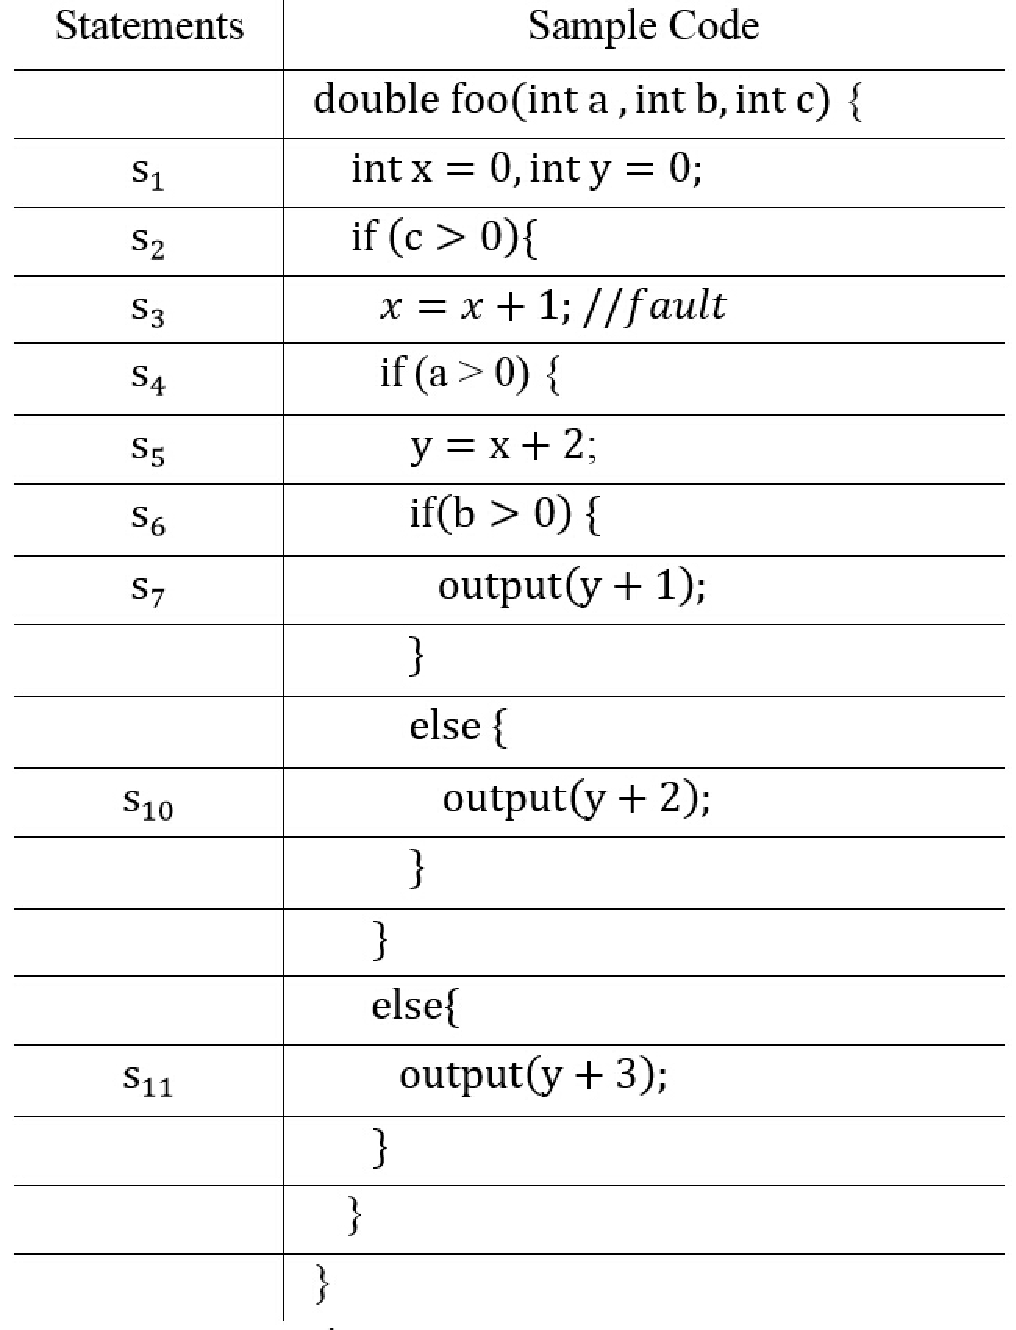
\includegraphics[width=0.6\textwidth]{chapter2_fig2.pdf}
\vspace {0em}\caption{Erroneous Program} \label{fig2.3}
\end{center}
\vspace {0em}
\end{figure}

Since model \eqref{eq7} does not adjust for confounding bias, $\widehat {\beta _1^*}$ may 
deviate from the failure causing effect of covering statement $s$.  For example, consider the program in Figure \ref{fig2.3}, which contains a faulty statement $s_3$, which should be $x=x+1$.  
Suppose that we want to estimate the failure causing effect of covering statement $s=s_7$.  
Assume that none of the observed executions cover statement $s_10$.  
This is a random violation of positivity, because $(T_{s_7}=0,C_{s_7}=1)$ is not observed.  
The estimator $\widehat{\beta_1^*}$ will be equal to $P(Y=1|C_{s_7}=1)$, where $pred({s_7})=s_6$.  
Because the faulty statement $s_3$ always executes before statement $s_6$ is executed, 
we have $P(Y=1|C_{{s_7}}=1)=1$, even though both $s_7$ and $s_6$ are correct.

To address random nonpositivity involving a target statement $s$ and $pred(s)$, 
we propose assigning the suspiciousness score of $pred(s)$ to statement $s$, 
provided that the causal effect estimator for $pred(s)$ adjusts for confounding.  
When random nonpositivity occurs, $s$ and $pred(s)$ have the same coverage information 
and thus their coverage-based suspiciousness scores should be same.  Referring again to Figure \ref{fig2.3}, 
the suspiciousness score of $s_7$ would be made equal to the suspiciousness score of $s_6$, 
which is estimated by model \eqref{eq1} with $T_s=s_6$ and $C_s=s_4$.  
We empirically evaluate this idea in Section \ref{sec4.2}.

\subsection{Analysis of RQ3}\label{sec3.3}
In this section, we will derive a probabilistic interpretation for causal effect estimator $\widehat{\beta_1}$.  
We first define some notation for different numbers of executions: $N_{T_s}=1$ is the number 
of executions with $T_s=1$; $N_{C_s}=1$ is the number with $C_s=1$; $N_{{C_s}=1,{T_s}=1}$ 
is the number with $C_s=1$ and $T_s=1$; $N_{{C_s}=1,Y=1}$ is the number with $C_s=1$ and $Y=1$; 
and $N_{{T_s}=1,Y=1}$ is the number with $T_s=1$ and $Y=1$.  Because $pred(s)$ dominates $s$ 
in the program’s control flow graph, we have
\begin{equation}\label{eq8}
N_{{C_s}=1,{T_s}=1}=N_{T_s=1}
\end{equation}
In addition, since $C_s$, $T_s$ are binary variables we have:
\begin{equation}\label{eq9}
{\mathbf{c_s}} \cdot {\mathbf{c_s}} = {\sum\nolimits_i {({c_{s,i}})} ^2} = {N_{C_s = 1}}
\end{equation}
\begin{equation}\label{eq10}
{\mathbf{c_s}} \cdot {\mathbf{t_s}} = {\mathbf{t_s}} \cdot {\mathbf{t_s}}
={\sum\nolimits_i {({t_{s,i}})} ^2} = {N_{T_s = 1}}
\end{equation}
\begin{equation}\label{eq11}
{\mathbf{c_s}} \cdot {\mathbf{y}} = {\sum\nolimits_i {c_{s,i}}y_i} = {N_{C_s= 1,Y=1}}
\end{equation}
\begin{equation}\label{eq12}
{\mathbf{t_s}} \cdot {\mathbf{y}} = {\sum\nolimits_i {t_{s,i}y_i}} = {N_{T_s= 1,Y=1}}
\end{equation}

With equations \eqref{eq8}-\eqref{eq12} we can rewrite the numerator \eqref{eq5} 
of the quotient in equation \eqref{eq3}, as
\begin{equation}\label{eq13}
\begin{array}{l}
N_{C_s=1}N_{T_s=1,Y=1}-N_{T_s=1}N_{C_s=1,Y=1}
-n{{\overline {\mathbf{c}_s}} ^2} N_{T_s=1,Y=1}
+n{\overline{\mathbf{c}_s}}{\overline{\mathbf{t}_s}}N_{C_s=1,Y=1}\\
=N_{C_s=1}N_{T_s=1,Y=1}-N_{T_s=1}N_{C_s=1,Y=1}
-\frac{{{N_{C_s=1}}^2}{N_{T_s=1,Y=1}}}{n}
+\frac{{N_{C_s=1}}{N_{T_s=1}}{N_{C_s=1,Y=1}}}{n}\\
=N_{C_s=1}N_{T_s=1,Y=1}(1-\frac{N_{C_s=1}}{n})-N_{T_s=1}N_{C_s=1,Y=1}(1-\frac{N_{C_s=1}}{n})\\
=(N_{C_s=1}N_{T_s=1,Y=1}-N_{T_s=1}N_{C_s=1,Y=1})(1-\frac{N_{C_s=1}}{n})
\end{array}
\end{equation}

Applying equations \eqref{eq8}-\eqref{eq12} to the denominator \eqref{eq6} in equation \eqref{eq3}, 
we can rewrite it as
\begin{equation}\label{eq14}
\begin{array}{l}
N_{C_s=1}N_{T_s=1}-{N_{T_s=1}}^2
-n{{\overline {\mathbf{t}_s}} ^2} N_{C_s=1}
-n{{\overline{\mathbf{c}_s}}^2}N_{T_s=1}
+2n{\overline{\mathbf{c}_s}}{\overline{\mathbf{t}_s}}N_{T_s=1}\\
=N_{C_s=1}N_{T_s=1}-{N_{T_s=1}}^2
-\frac{{{N_{T_s=1}}^2}{N_{C_s=1}}}{n}
-\frac{{{N_{C_s=1}}^2}{N_{T_s=1}}}{n}
+\frac{2N_{C_s=1}N_{T_s=1}}{n}\\
=N_{C_s=1}N_{T_s=1}-{N_{T_s=1}}^2+\frac{{{N_{T_s=1}}^2}{N_{C_s=1}}-{{N_{C_s=1}}^2}{N_{T_s=1}}}{n}\\
=N_{T_s=1}(N_{C_s=1}-N_{T_s=1})(1-\frac{N_{C_s=1}}{n})
\end{array}
\end{equation}

Given the derivations in \eqref{eq13} and \eqref{eq14}, equation \eqref{eq3} can be rewritten as follows:
\begin{equation}\label{eq15}
\begin{array}{l}
\widehat {\beta _1}=\frac{(N_{C_s=1}N_{T_s=1,Y=1}-N_{T_s=1}N_{C_s=1,Y=1})(1-\frac{N_{C_s=1}}{n})}{N_{T_s=1}(N_{C_s=1}-N_{T_s=1})(1-\frac{N_{C_s=1}}{n})}\\
=\frac{N_{C_s=1}N_{T_s=1,Y=1}-N_{T_s=1}N_{C_s=1,Y=1}}{N_{T_s=1}(N_{C_s=1}-N_{T_s=1})}\\
=\frac{N_{C_s=1}N_{T_s=1,Y=1}-N_{T_s=1}N_{T_s=1,Y=1}}{N_{T_s=1}(N_{C_s=1}-N_{T_s=1})}
-\frac{N_{T_s=1}N_{C_s=1,Y=1}-N_{T_s=1}N_{T_s=1,Y=1}}{N_{T_s=1}(N_{C_s=1}-N_{T_s=1})}\\
=\frac{N_{T_s=1,Y=1}}{N_{T_s=1}}-\frac{N_{C_s=1,Y=1}-N_{T_s=1,Y=1}}{N_{C_s=1}-N_{T_s=1}}
\end{array}
\end{equation}
Thus, the causal effect estimator $\widehat{\beta_1}$ is a difference of two terms:
\begin{equation}\label{eq16}
\frac{N_{T_s=1,Y=1}}{N_{T_s=1}}
\end{equation}
and
\begin{equation}\label{eq17}
\frac{N_{C_s=1,Y=1}-N_{T_s=1,Y=1}}{N_{C_s=1}-N_{T_s=1}}
\end{equation}
Let $N_{T_s=0,C_s=1}$ be the number of executions with $(T_s=0,C_s=1)$, and let $N_{T_s=0,C_s=1,Y=1}$ be the number of executions with $(T_s=0,C_s=1,Y=1)$.  Considering the relationship between $s$ and $pred(s)$, we see that
\begin{equation}\label{eq18}
N_{T_s=0,C_s=1}=N_{C_s=1}--N_{T_s=1}
\end{equation}
\begin{equation}\label{eq19}
N_{T_s=0,C_s=1,Y=1}=N_{C_s=1,Y=1}--N_{T_s=1,Y=1}
\end{equation}
Recall that $N_{C_s=1,T_s=1}=N_{T_s=1}$. Similarly, we have $N_{T_s=1,Y=1}=N_{C_s=1,T_s=1,Y=1}$.  Rewriting term \eqref{eq16}, we see that
\begin{equation}\label{eq20}
\begin{array}{l}
\frac{N_{T_s=1,Y=1}}{N_{T_s=1}}=\frac{\frac{N_{C_s=1,T_s=1,Y=1}}{n}}{\frac{N_{T_s=1}}{n}}\\
\approx \frac{P(T_s=1,C_s=1,Y=1)}{P(T_s=1,C_s=1)}\\
=P(Y=1|T_s=1,C_s=1)
\end{array}
\end{equation}
Applying equations \eqref{eq18} and \eqref{eq19} to term \eqref{eq17}, we see that
\begin{equation}\label{eq21}
\begin{array}{l}
\frac{N_{C_s=1,Y=1}-N_{T_s=1,Y=1}}{N_{C_s=1}-N_{T_s=1}}=\frac{\frac{N_{T_s=0,C_s=1,Y=1}}{n}}{\frac{N_{T_s=0,C_s=1}}{n}}\\
\approx \frac{P(T_s=0,C_s=1,Y=1)}{P(T_s=0,C_s=1)}\\
=P(Y=1|T_s=0,C_s=1)
\end{array}
\end{equation}
Hence,
\begin{equation}\label{eq22}
\widehat {\beta _1} \approx P(Y=1|T_s=1,C_s=1)-P(Y=1|T_s=0,C_s=1)
\end{equation}
This demonstrates that Baah et al’s AFCE estimator $\widehat{\beta_1}$ 
actually approximates the {\it associational risk difference} \cite{hernan2004definition} within 
the stratum of executions with $C_s=1$.  This measure is equal to the 
{\it causal risk difference} \cite{crump2006moving} within the stratum $C_s=1$ if the treatment 
effect of $T_s$ on $Y$ is unconfounded in that stratum.  Whether or not the 
last condition is true, $\widehat{\beta_1}$ is not an unbiased estimator of the 
AFCE over the whole population of executions.  This is consistent with our conclusions about structural nonpositivity in Section \ref{sec3.1}.  Note that if a random violation of positivity occurs, one of the two probability terms in equation \eqref{eq22} will be undefined, so $\widehat{\beta_1}$ will be undefined.

\section{Empirical Study}
We also conducted an empirical study of research questions RQ2 and RQ3.  We first describe the study platform and subject programs and then present the study results.


\subsection{Study Platform and Subject Programs}
{\bf Platform}: Our study platform is based on the JavaPDG dependence analysis tool \cite{shu2013javapdg} and the ASM Java bytecode manipulation framework \cite{ASM}.  To obtain the data required to use Baah et al’s model \eqref{eq1}, we first instrument a Java subject program’s class files using ASM, to record statement coverage information at runtime.  Then JavaPDG is used to generate a program dependence graph (PDG) of the subject program.  Each PDG node is mapped back to a source code statement.  For each statement , the PDG records the statement ID of $pred{s}$, if the latter exists.

{\bf Subject Programs}: We selected three subject programs written in Java: NanoXML, Rome, and Xerces2.  NanoXML \cite{Nanoxml} (version 1) is an XML parser from Software-artifact Infrastructure Repository (SIR) \cite{SIR}.  Rome (revision 840) is a open source library for parsing, generating, and publishing RSS and Atom feeds \cite{Rome}.  Apache Xerces2(v.2.9.1) is a processor for parsing, validating, serializing, and manipulating XML \cite{Xerces2}.  

{\bf Tests and Faults}: NanoXML comes with test suites.  To test Xerces2, XML files were collected from the system directories of an Ubuntu Linux 7.04 machine.  For Rome, test cases were obtained by downloading Atom and RSS files with a custom web crawler.  A sample of faults was selected randomly from the repository for each subject program: 4 for NanoXML, 5 for Rome, and 5 for Xerces2.  A summary of our subject programs and tests is shown in Table \ref{table1}.  

\begin{table}
\caption{Subject programs, tests, and faults}\label{table1}
\centering
\begin{tabular}{|c|c|c|c|}
\hline
Subject Program	&	LOC	&	Number of Tests	&	Faults	\\ \hline
NanoXML (SIR v1)	&	4.4K	&	1,000	&	4	\\ \hline
Rome (revision 840)	&	24K	&	2,000	&	5	\\ \hline
Xerces2 (v.2.9.1)	&	167K	&	1536	&	5	\\ \hline

\end{tabular}
\end{table}


\subsection{Evaluation of RQ2}\label{sec4.2}

To evaluate our conclusions about RQ2, we designed two sub-studies. The first sub-study was done to check whether random violations of positivity happen in practice. For a statement , such violations might occur in two ways: (1) no test executions have $(T_s=0,C_s=1)$, which means $s$ is always covered given $C_s=1$ and (2) no test executions have $(T_s=1,C_s=1)$, which means $s$ is never covered given $C_s=1$.  Note that in case (2), statement $s$ is never executed and so will not be assigned a suspiciousness score.  Thus, in our study we considered only case (2).  We also considered {\it only} statements $s$ for which $pred{s}$ exists.  Then we determined, for each subject program, which such statements were covered.  For each covered statement $s$, we checked if there were executions with $(T_s=0,C_s=1)$.  If not, a random violation of positivity, denoted RVP, occurred for $s$.  Table \ref{table2} shows the proportion of RVP statements among all covered statements for each subject program.  It shows that 4\% to 7\% of covered statements had random violations of positivity.

\begin{table}
\caption{Proportion of RVP statements among Covered statements with forward control dependence predecessor}\label{table2}
\centering
\begin{tabular}{|c|c|c|c|}
\hline
Subject Program	&	Number of RVP	&	Covered Statements	&	Proportion	\\ 
 & statements & with $pred(s)$ &\\\hline
NanoXML	&	19&	315	&	6.03\%	\\ \hline
Rome 	&	95	&	1353	&	7.02\%	\\ \hline
Xerces2 &	232	&	5545	&	4.18\%	\\ \hline

\end{tabular}
\end{table}

The second sub-study for RQ2 was done to determine if random violations of positivity affect the suspiciousness scores of statements.  The performance of Baah et al’s causal effect estimator $\widehat{\beta_1}$ was measured by the number of RVP statements assigned a ``bad" suspiciousness score.  We considered an RVP statement to have a bad suspiciousness score if its score was larger than  but the statement was not faulty or if its score was at most  but the statement was faulty.  In Section \ref{sec3.2}, we proposed assigning the suspiciousness score of $pred{s}$ to an RVP statement $s$.  Hence, we also checked if this ``adjusted" estimator performed better than $\widehat{\beta_1}$ under random violations of positivity.  Table \ref{table3} shows the number of RVP statement assigned “bad” suspiciousness scores by each estimator.  All the RVP statements of NanoXML had ``bad" suspiciousness scores.  For Xerces2, 207 out of 232 RVP statements had bad suspiciousness scores.  For Rome, RVP statements do not cause big problem: only 29 out of 95 RVP statements had bad suspiciousness scores.  When we applied the adjusted causal effect estimator, the numbers of RVP statements with bad suspiciousness scores dropped to 3 for NanoXML, to 23 for Rome, and to 102 for Xerces2.  The results suggest that the adjusted estimator performs better than the original one under random violations of positivity.
\begin{table}
\caption{Comparison between Baah et al’s  Original estimator and the ``Adjusted” estimator}\label{table3}
\centering
\begin{tabular}{|c|c|c|c|}
\hline
Subject Program	&	Number of RVP	&	Baah et al’s	&	Adjusted	\\ 
 & statements & estimator-bad scores &estimator-bad scores\\\hline
NanoXML	&	19&	19	&	3	\\ \hline
Rome 	&	95	&	29	&	23	\\ \hline
Xerces2 &	232	&	207	&	102	\\ \hline

\end{tabular}
\end{table}

\subsection{Evaluation of RQ3}
In Section \ref{sec3.3}, we have derived equation \eqref{eq22}, which is a probabilistic characterization of Baah et al’s estimator $\widehat{\beta_1}$.  An alternative estimator can be computed based directly on the right side of this equation, by replacing each probability by the corresponding sample proportion.  The two estimators should produce nearly identical suspiciousness scores.  To evaluate the correctness of equation \eqref{eq22}, we applied both estimators to the data from each of the subject programs.  We then computed the mean difference between these resulting scores, over all the statements of each subject program.  The result is shown in Table \ref{table4}.  We see that the mean difference is extremely small for each program, as is the variance of the difference.  Table \ref{table4} also shows the P-values of Student’s  tests of the null hypothesis of no difference in the score distributions, which are all 1 for each program. This indicates the means of each two groups of suspiciousness scores are statistically indistinguishable.

\begin{table}
\caption{Comparison between Baah et al’s  Original estimator and the ``Adjusted” estimator}\label{table4}
\centering
\begin{tabular}{|c|c|c|c|}
\hline
Subject Program	&	Mean	&	Variance	&	P-value	\\ \hline
NanoXML 	&	1.68E-16	&	1.25E-29	&	1	\\ \hline
Rome 	&	5.68E-16	&	8.05E-29	&	1	\\ \hline
Xerces2 	&	1.79E-16	&	7.64E-29	&	1	\\ \hline

\end{tabular}
\end{table}

We also measured the computation time for both estimators. The results are shown in Table \ref{table5}.  The probability-based causal effect estimator required substantially less computation time than the regression-based estimator, especially for the large subject program Xerces2.  

\begin{table}
\caption{Average execution times of regression-based causal effect estimator and probability-based causal effect estimator}\label{table5}
\centering
\begin{tabular}{|c|c|c|c|}
\hline
Subject Program	&	Regression	&	Probability	\\ \hline
NanoXML 	&	8.049 sec	&	4.354 sec	\\ \hline
Rome 	&	135.809 sec	&	44.308 sec	\\ \hline
Xerces2 	&	143.235 sec	&	54.578 sec	\\ \hline

\end{tabular}
\end{table}

\section{Related Work}
The most closely related work is on causal statistical fault localization techniques.  Baah et al \cite{baah2011mitigating} extended their original CSFL model by also controlling for confounding bias caused by data flow dependences, and they found this reduced localization costs.  Gore et al \cite{gore2012reducing} proposed an improved version of Baah et al’s original approach by providing a model that also addresses what they call {\it failure flow confounding bias}.  Shu et al \cite{shu2013mfl} proposed a CSFL technique for localizing faulty {\it methods} in large programs, which exploits dynamic call graph and dependence information and addresses nonpositivity.

Other related work examines positivity violations in causal inference generally.  Westreich, et al \cite{westreich2010invited} pointed out that positivity is important for making valid inferences from observational data but is often overlooked in practice, and they discussed general ways of dealing with nonpositivity.  Wang, et al \cite{wang2006diagnosing} analyzed the bias of an inverse-probability-of-treatment-weighted estimator in the face of positivity violations.  Petersen, et al \cite{petersen2010diagnosing} systematically reviewed how violations of positivity influence different types of causal-effect estimators.

Some recent studies have investigated methods for estimating causal effects in the presence of positivity violations. A ``trimming” technique is used in \cite{crump2006moving} is to discard units whose probability of treatment, conditional on covariates, is outside of a specified interval.  Another method proposed by Bembom et al  \cite{bembom2008data} is to exclude the confounders involved in positivity violations from the adjustment sets.  

\section{Conclusion}
Causal statistical fault localization techniques such as Baah et al’s CSFL regression technique can be biased when the positivity condition is violated \cite{bai2015importance}.  In this paper, we have analyzed two types of violations of positivity: structural violations and random violations. We established that structural violations do occur with Baah et al’s technique but are not harmful.  We proved that random violations also occur and that they can distort suspiciousness scores.  To address the problem of random nonpositivity, we proposed a modification to the way suspiciousness scores are assigned with Baah et al.’s technique.  Empirical results were presented that indicate it improves the technique’s performance. We also presented a probabilistic characterization of Baah et al’s estimator and showed that it provides a more efficient way to compute the same scores. Since Baah et al’s CSFL regression technique is based on a causal graph which omits data dependences, and since it characterizes program states only in terms of statement coverage, it does not eliminate all confounding bias in fault localization.  Nevertheless, it seems to perform well, and with our suggested improvements it is computationally efficient.










